%!TEX root = ../main.tex

\addchap{Anhang}
\begin{itemize}
	\item Schaltplan Seite 1 (Übersicht) 				\dotfill{} \pageref{apx:sp_uebersicht}
	\item Schaltplan Seite 2 (Stromversorgung) 			\dotfill{} \pageref{apx:sp_power}
	\item Schaltplan Seite 3 (Mikrocontroller) 			\dotfill{} \pageref{apx:sp_uC}
	\item Schaltplan Seite 4 (Serielle Schnittstellen) 	\dotfill{} \pageref{apx:sp_seriell}
	\item Schaltplan Seite 5 (Sonstiges) 				\dotfill{} \pageref{apx:sp_div}
	\item Übersicht Layout 								\dotfill{} \pageref{apx:bs_1}
	\item Layerstackup 									\dotfill{} \pageref{apx:bs_2}
\end{itemize}

\newcommand{\myscale}{0.8}
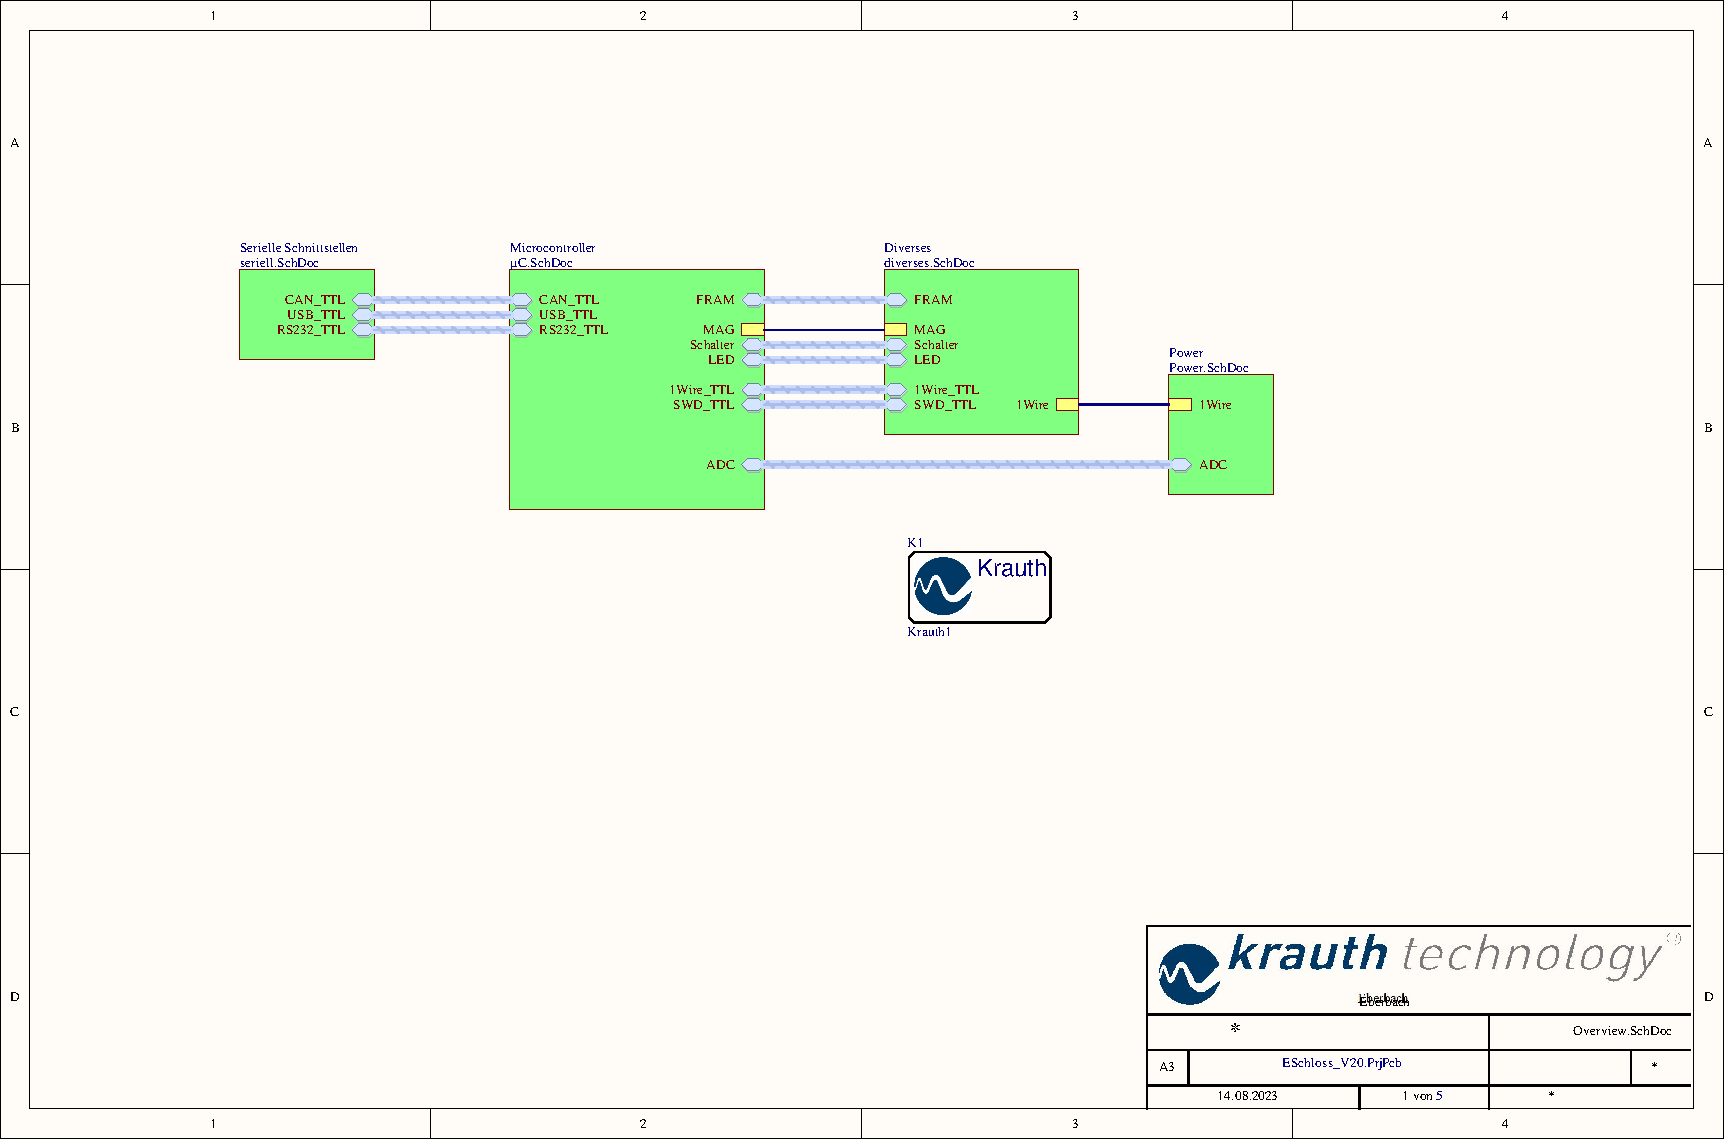
\includepdf[scale=\myscale, offset= 0mm -3mm, landscape=true, pages=1, pagecommand={\label{apx:sp_uebersicht}}]{resources/ESchloss_V20_sp.pdf}
\includepdf[scale=\myscale, offset= 0mm -3mm, landscape=true, pages=2, pagecommand={\label{apx:sp_power}}]{resources/ESchloss_V20_sp.pdf}
\includepdf[scale=\myscale, offset= 0mm -3mm, landscape=true, pages=3, pagecommand={\label{apx:sp_uC}}]{resources/ESchloss_V20_sp.pdf}
\includepdf[scale=\myscale, offset= 0mm -3mm, landscape=true, pages=4, pagecommand={\label{apx:sp_seriell}}]{resources/ESchloss_V20_sp.pdf}
\includepdf[scale=\myscale, offset= 0mm -3mm, landscape=true, pages=5, pagecommand={\label{apx:sp_div}}]{resources/ESchloss_V20_sp.pdf}

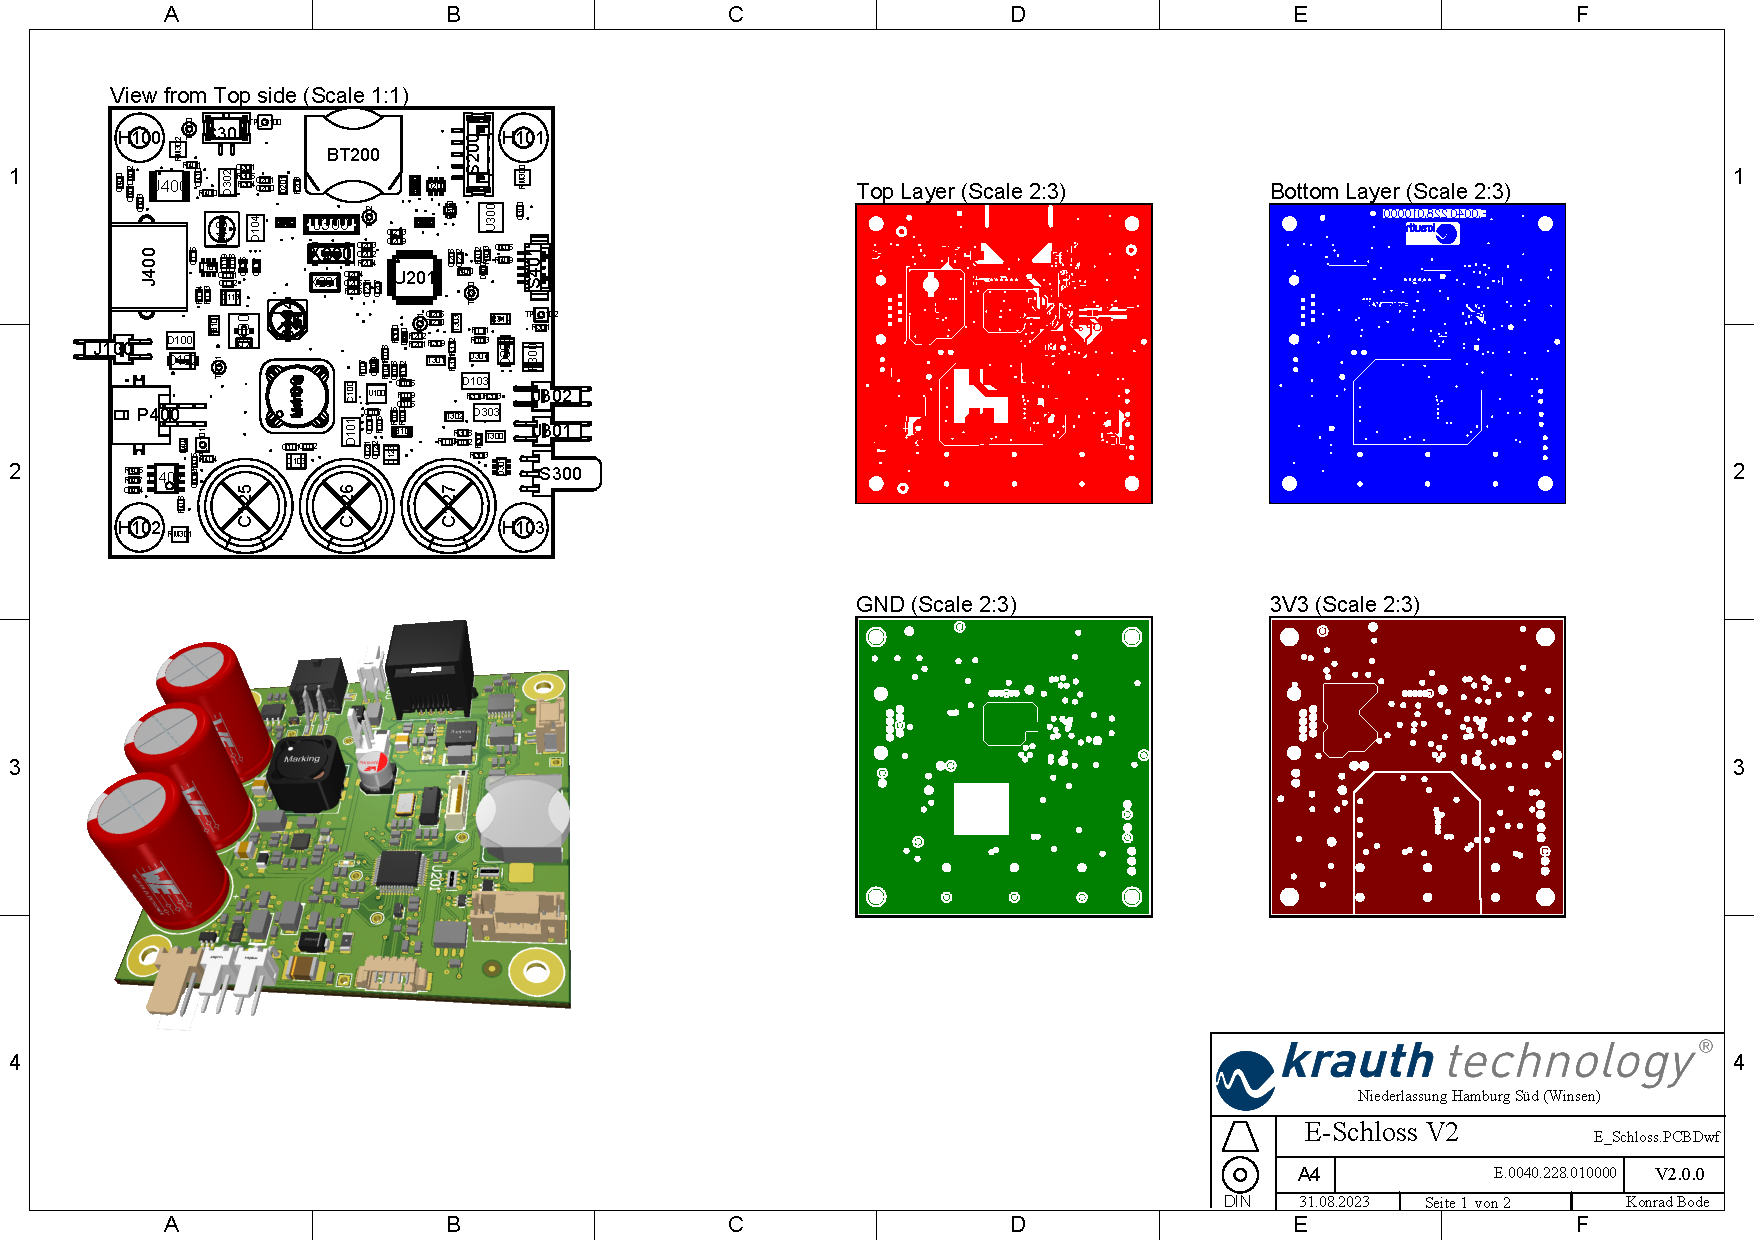
\includepdf[scale=\myscale, offset= 0mm -3mm, landscape=true, pages=1, pagecommand={\label{apx:bs_1}}]{resources/ESchloss_V20_bs.pdf}
\includepdf[scale=\myscale, offset= 0mm -3mm, landscape=true, pages=2, pagecommand={\label{apx:bs_2}}]{resources/ESchloss_V20_bs.pdf}